\setlength{\footskip}{8mm}

\chapter{Preliminary Prototype}
\label{ch:methodology}

\textit{This chapter describes an experiment and shows the preliminary prototype of wrong-way driving detection system.}

\section{System Overview}

The proposed system is designed for study possible ways to detect wrong-way driving. This system aims to estimate motion for rigid 3D objects moving parallel to a ground plane. The system consists of 2 parts: motion estimation part and learning part. The workflow of the system is shown in Figure~\ref{fig:System workflow}.  

\begin{figure}[t]
	\centering
	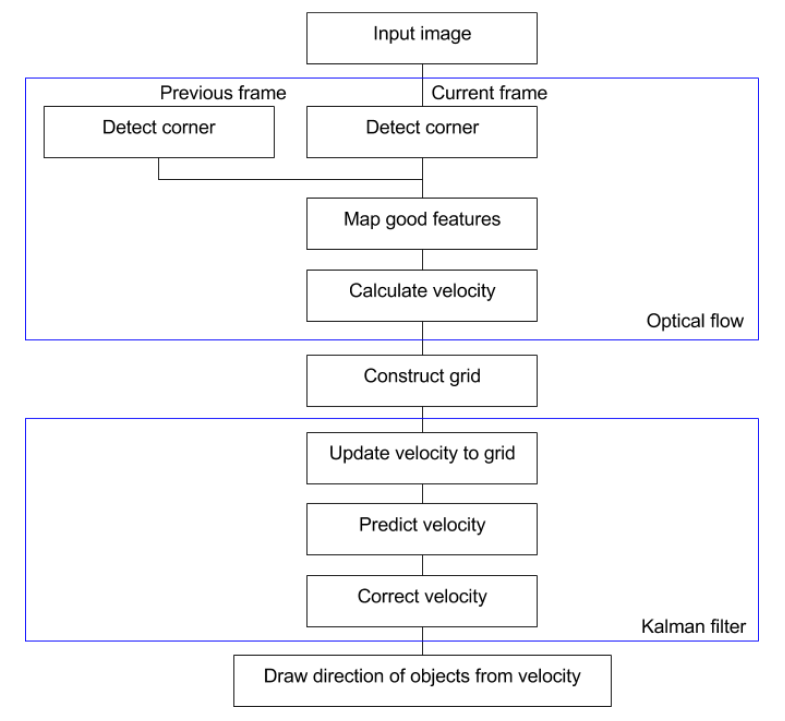
\includegraphics[width=6in]{figures/workflow.jpg}  
	\caption[System workflow]{ System workflow.}
	\label{fig:System workflow}
\end{figure}

\section{Motion Estimation (Optical flow)}
The detection and motion estimation in this system is based on Optical flow. It looks for corners in image and tags its as a good feature. The good features from two frames (previous frame and current frame) are mapped. Then, we can see a motion of the object. In Figure~\ref{fig:opticalflowExample} shows motion detection of vehicles on the road. 

\begin{figure}[t]
	\centering
	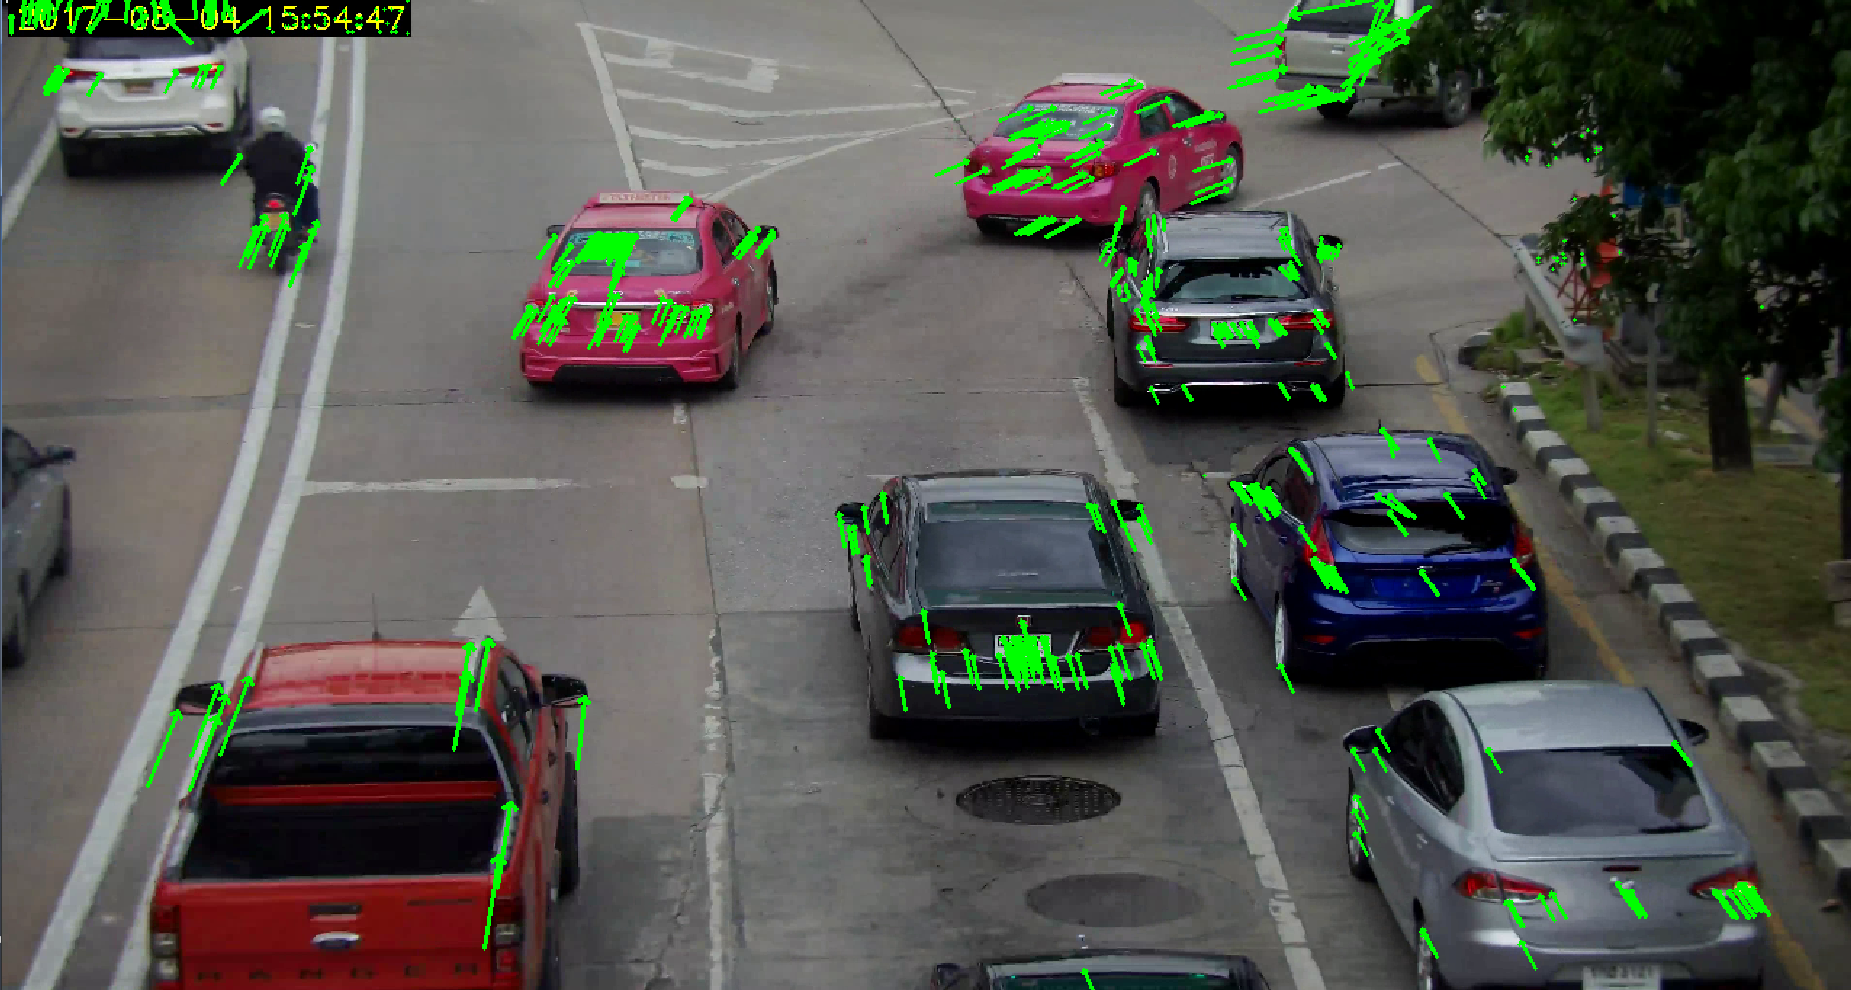
\includegraphics[width=6in]{figures/opticalflowExample.jpg}  
	\caption[The result of Optical flow]{The result of Optical flow.}
	\label{fig:opticalflowExample}
\end{figure}

\section{Learning (Kalman filter)}
We process at image size is $1280 \times 720$ pixels 

\begin{figure}[t]
	\centering
	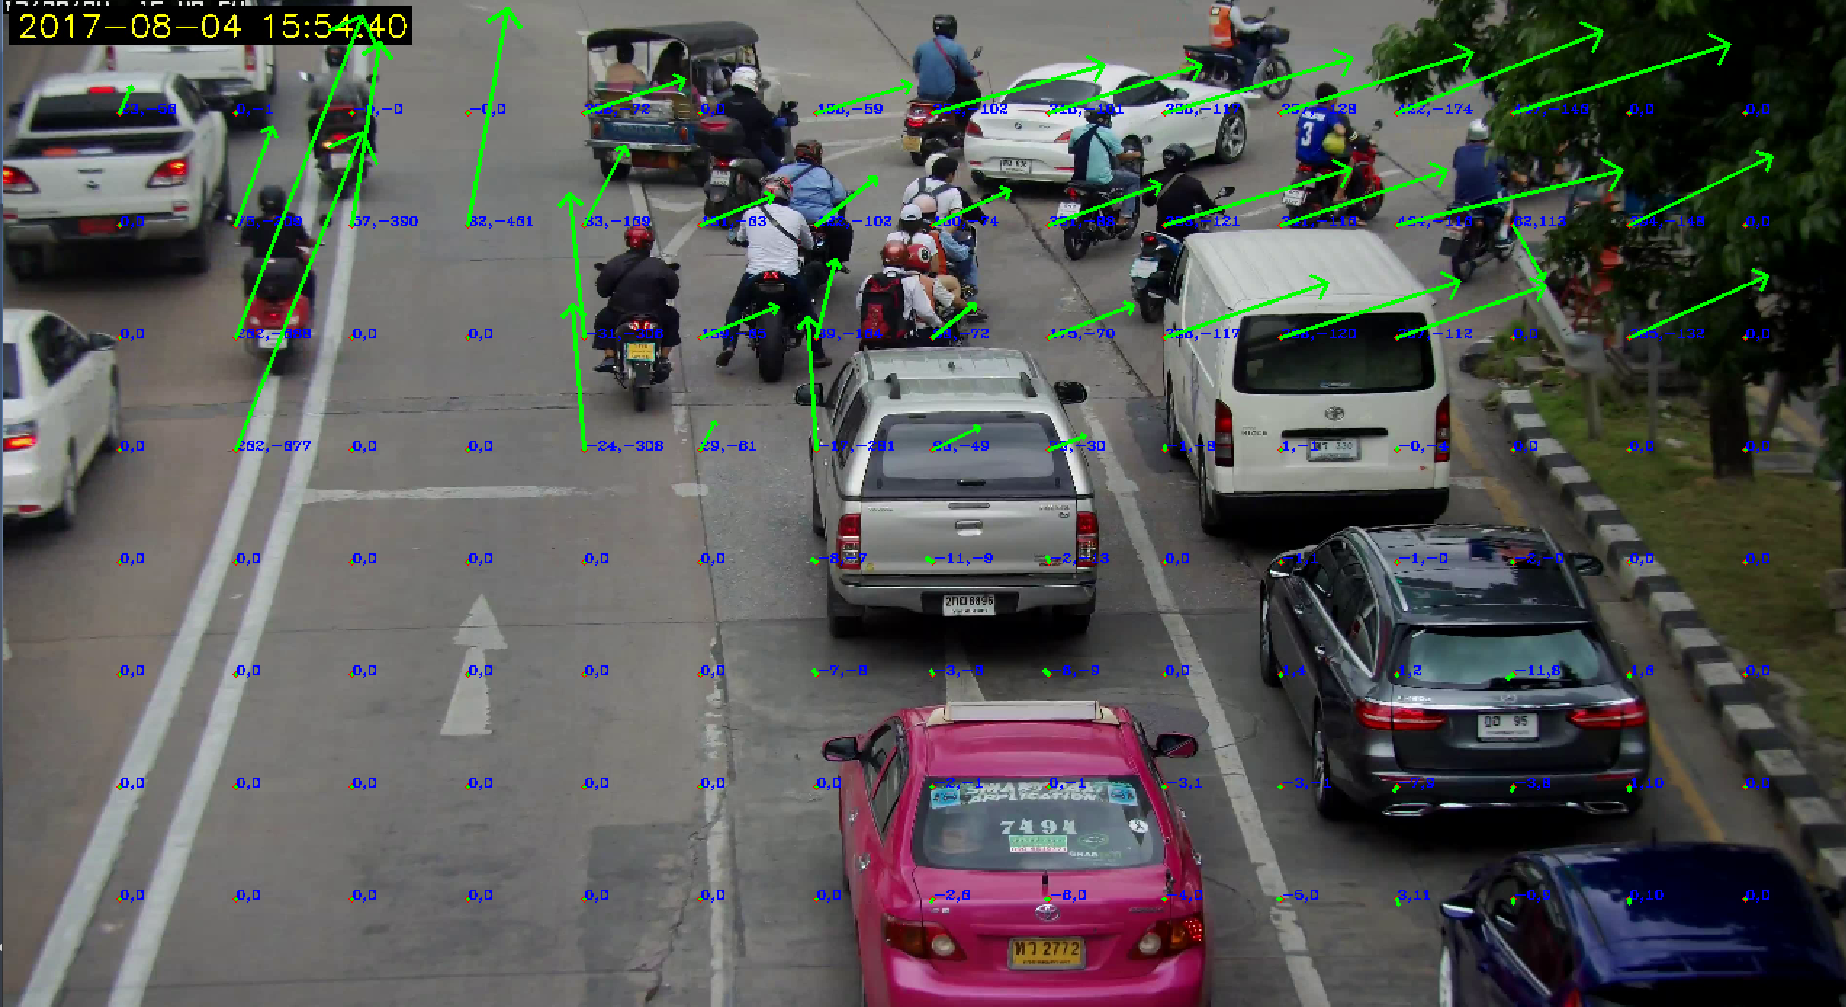
\includegraphics[width=6in]{figures/kalmanResult.jpg}  
	\caption[Direction from learning velocity]{Direction from learning velocity.}
	\label{fig:kalmanResult}
\end{figure}

\begin{figure}[t]
	\centering
	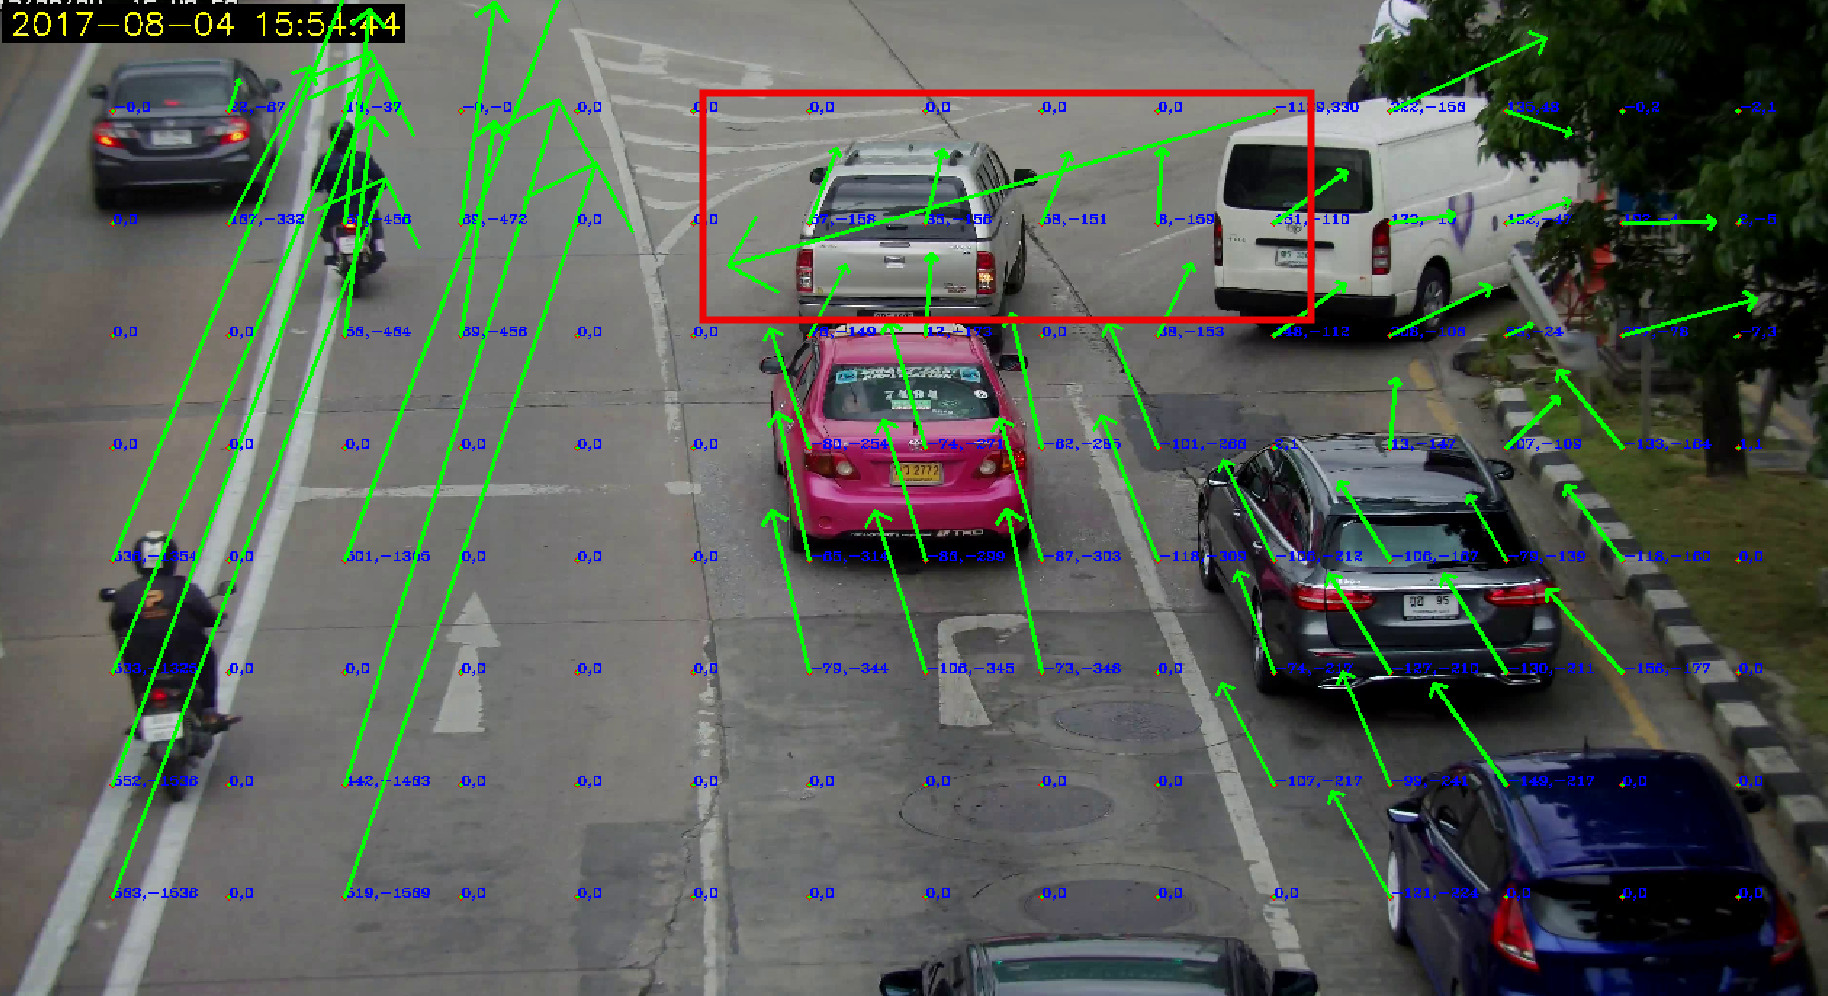
\includegraphics[width=6in]{figures/errorfromOF.jpg}  
	\caption[The error of the system]{The error of the system.}
	\label{fig:errorfromOF}
\end{figure}

\FloatBarrier

